%%% ---- スライドの場合 (start) remove comment out
\documentclass[t,dvipdfmx,10pt]{beamer}
\newcommand*{\kougi}{slide}   % kougi is slide
%%%  ---- スライドの場合 (stop)

%%% ---- from https://eqseqs.hatenablog.com/entry/2018/09/09/214453 
\usepackage{zxjatype}
\usepackage[ipa]{zxjafont}
\usepackage{caption} 
\usepackage{algorithmic}
\usepackage{algorithm}
\usepackage{amsmath}
\usepackage[absolute,overlay]{textpos}

%%% 

% ---- スタイル設定 (start) 
\usepackage{ifthen}
\usepackage{otf}
\usepackage[varg]{txfonts}
\usepackage{mediabb}
\usepackage[absolute,overlay]{textpos}
\usepackage{amsthm}
\usepackage{tcolorbox}
\tcbuselibrary{theorems}
\newtheorem{dfn}{定義}
\newtheorem{thm}{定理}
\uselanguage{japanese}
\languagepath{japanese}
\deftranslation[to=japanese]{Theorem}{定理}
\deftranslation[to=japanese]{Lemma}{補題}
\deftranslation[to=japanese]{Example}{例}
\deftranslation[to=japanese]{Examples}{例}
\deftranslation[to=japanese]{Definition}{定義}
\deftranslation[to=japanese]{Definitions}{定義}
\deftranslation[to=japanese]{Problem}{問題}
\deftranslation[to=japanese]{Solution}{解}
\deftranslation[to=japanese]{Fact}{事実}
\deftranslation[to=japanese]{Proof}{証明}
\def\proofname{証明}
%\usepackage{hyperref}
%\usepackage{pxjahyper}
%\usetheme{Frankfurt}%Frankfurt,AnnArbor, Antibes, Berlin, Berkeley, Bergen, Boadilla, boxes, Copenhagen

%\beamerdefaultoverlayspecification{<+->}% 箇条書きを段階的にみせたいとき
%\setbeamercovered{transparent}%隠してるアイテムを半透明で表示
%\renewcommand{\kanjifamilydefault}{\gtdefault}%日本語フォントをゴシックに
\usepackage{graphicx}% 各種画像の張り込み

%\usepackage[english]{babel}%多言語文書を作成する
\usepackage{amsmath,amssymb}%標準数式表現を拡大する

%デザインの選択(省略可)
%\usetheme{Luebeck}
%\usetheme{CambridgeUS}
%\usetheme{Copenhagen}
\usetheme[progressbar=frametitle]{metropolis}
%\usetheme[hideothersubsections]{Goettingen}
%\usetheme{Goettingen}

%\usetheme{Hannover}
%カラーテーマの選択(省略可)
\usecolortheme{orchid}
%フォントテーマの選択(省略可)
\usefonttheme{professionalfonts}
%フレーム内のテーマの選択(省略可)
\useinnertheme{circles}
%フレーム外側のテーマの選択(省略可)
\useoutertheme{infolines}
%しおりの文字化け解消
\usepackage{atbegshi}
\ifnum 42146=\euc"A4A2
\AtBeginShipoutFirst{\special{pdf:tounicode EUC-UCS2}}
\else
\AtBeginShipoutFirst{\special{pdf:tounicode 90ms-RKSJ-UCS2}}
\fi
%ナビゲーションバー非表示
\setbeamertemplate{navigation symbols}{}
%タイトル色
\setbeamercolor{title}{fg=structure, bg=}
%フレームタイトル色
\setbeamercolor{frametitle}{fg=structure, bg=}

% caption に番号追加
\setbeamertemplate{caption}[numbered]
% caption 日本語
\renewcommand{\figurename}{図}
\renewcommand{\tablename}{表}

\usepackage[export]{adjustbox} % loads also graphicx


% ---- スタイル設定 (stop) 

% ---- 内容設定 (start) 
\title[自主ゼミ]{「ニューラルネットワークと機械学習」勉強会}
\subtitle{CHAPTER1 ニューラルネットワークを用いた手書き文字認識}
\author[Kimihiro Doi]{土井 公宏}
\institute{}
\date[]{2021/04/08}
\subject{\LaTeX{}+Beamer} % just for pdf info
% ---- 内容設定 (stop) 

\begin{document}
% ---- タイトルと目次、スライドの場合 (start) 
\begin{frame}
 \titlepage 
\end{frame}

\begin{frame}<beamer>
  \frametitle{目次}
    \tableofcontents[] 
%  \tableofcontents[hideothersubsections] % hide subsection
\end{frame}


% 内容

\section{パーセプトロンとシグモイドニューロン}
\begin{frame}{パーセプトロン}
\begin{textblock*}{0.09\linewidth}(40pt, 220pt)
    \centering
    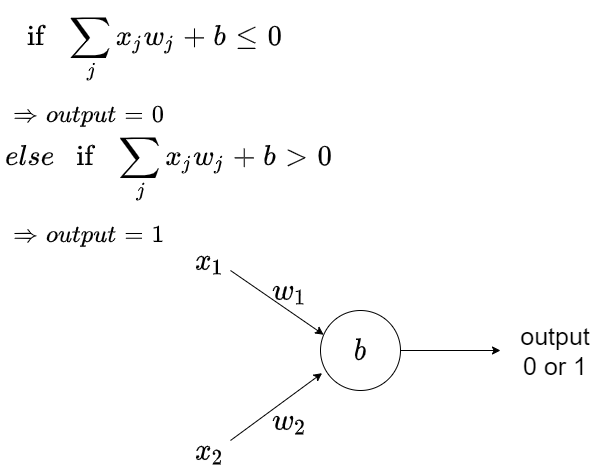
\includegraphics[width=\linewidth]{./パーセプトロン.png}
    
\end{textblock*}
    
\end{frame}
\begin{frame}
\frametitle{シグモイドニューロン}
\begin{itemize}
    \item シグモイドニューロンを組み合わせたものをニューラルネットワークと呼ぶ
    \item パーセプトロンの組み合わせでは得られない高い表現力をもつ
\end{itemize}
\begin{textblock*}{0.06\linewidth}(20pt, 230pt)
    \centering
    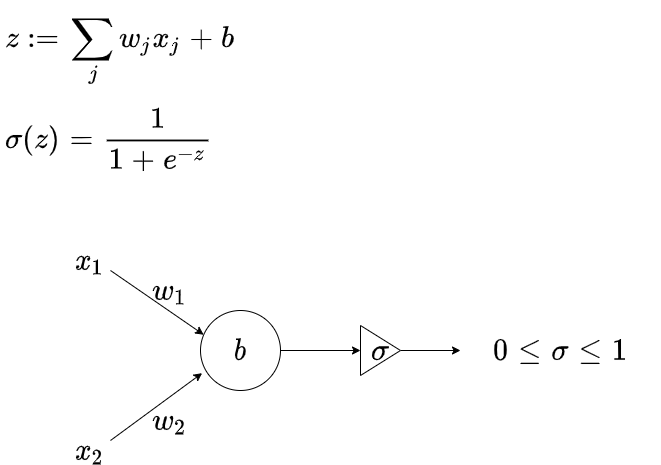
\includegraphics[width=\linewidth]{./sigmoid.png}
    
\end{textblock*}
\end{frame}
\begin{frame}{Exercises シグモイドニューロンのシミュレーション パート1}
\begin{block}{問題}
パーセプトロンを組み合わせたネットワークにおいて、すべての重みとバイアスを$c$倍しても挙動が変わらないことを示せ
\end{block}
ネットワークの挙動は,各パーセプトロンの出力によって決まるから,パーセプトロンの出力に変化がないことを示せばよい.$\sum_j cw_j x_j+cb=c(\sum_j w_j x_j+b)$であり,もとのパーセプトロンと正負が一致し,出力に変化はない.示すべきことが言えた.
\end{frame}
\begin{frame}{Exercises シグモイドニューロンのシミュレーション パート2}
\begin{block}{問題}
シグモイドニューロンを組み合わせたネットワークにおいて、$\sum wx+b\neq 0$であれば,すべての重みとバイアスを$\infty$倍すると,パーセプトロンの場合と同じ挙動をすることを示せ
\end{block}  
\begin{itemize}
    \item $z=\sum wx+b>0$の場合,$z=\infty$より$\sigma(z)=\frac{1}{1+e^{-z}}=\frac{1}{1+0}=1$となり,パーセプトロンの場合と一致する.
    \item $z=\sum wx+b<0$の場合,$z=-\infty$より$\sigma(z)=\frac{1}{1+e^{-z}}=\frac{1}{1+\infty}=0$となり,パーセプトロンの場合と一致する.
    \item $z=\sum wx+b=0$の場合,$z=0$より$\sigma(z)=\frac{1}{1+e^{-z}}=\frac{1}{1+1}=\frac{1}{2}$となり,パーセプトロンの場合(output=0)と一致しない.
\end{itemize}
示すべきことが言えた.
\end{frame}
\section{指数関数,対数関数,ベキ関数}
\begin{frame}{指数関数}
\begin{displaymath}
e^{z}=e^{x}(\cos y+i\sin y)
\end{displaymath}
と表せる.よって$|e^{z}|=e^{x}$であり,実部を即座に計算できる.
\begin{block}{問題}
$e^{z}=1$を満たす$z$を求めよ
\end{block}
$z$の実部は$|e^{z}|=1$より$e^{x}=1$を見たす$x$だから0である.よって$z=iy$と表せる.よって,$e^{z}=e^{iy}=\cos y+i\sin y=1$であり,$y=2n\pi$.
$z=2n\pi i$
\end{frame}

\begin{frame}{対数関数}
複素対数関数は多対一の写像であることに注意する.
\begin{block}{問題}
$z_1=-1+\sqrt 3 i$の自然対数を求めよ
\end{block}
$|z_1|=r_1=\sqrt {(-1)^2+(\sqrt 3)^2}=2$
\\
$\arg z_1=\theta_1=\frac{2}{3} \pi$(単位円を描くとわかる)
よって$z_1=\log 2e^{i\frac{2}{3}\pi}$
\\
$\log z_1=\log(-1+\sqrt 3 i)$=\log 2e^{i\frac{2}{3}\pi}=\log 2+i(\frac{2}{3}\pi+2n\pi)$

\end{frame}
\begin{frame}{ベキ関数}
\begin{block}{問題}
$i^{i}$を計算せよ
\end{block}
$i^{i}=e^{i\log i}=e^{i\log (1e^{\frac{\pi}{2}i})}=e^{i(\log 1+(\frac{\pi}{2}+2n\pi)i)}$
\end{frame}
\section{三角関数}
\begin{frame}{複素逆三角関数}
\begin{block}{問題}
$\sin^{-1}z$ を計算せよ
\end{block}
$z=\sin w=\frac{e^{iw}-e^{-iw}}{2i}$
\\
$\Leftrightarrow (e^{iw})^2-2ize^{iw}-1=0$
\\これを二次方程式とみてとくと
\\$e^{iw}=iz\pm\sqrt{1-z^2}$
\\複素数のルートは$\pm$がつくから,
\\$e^{iw}=iz+\sqrt{1-z^2}$
\\$w=-i\log(iz+\sqrt{1-z^2)}$
\end{frame}
\end{document}
